\documentclass[a4paper]{article}
\usepackage[utf8]{inputenc}
\usepackage[T1]{fontenc}
\usepackage{satex}

\title{Satex test}
\author{Samuel Mimram}

\deftwocell[cap,arrow]{cap : 0 -> 2}
\deftwocell[cup,arrow]{cup : 2 -> 0}
\deftwocell[circle]{eps : 1 -> 0}
\deftwocell[circle]{eta : 0 -> 1}
\deftwocell[circle]{sigma : 1 -> 1}
\deftwocell[triangle]{mu : 2 -> 1}
\deftwocell[triangle]{delta : 1 -> 2}
\deftwocell[cap,arrow=left]{I : 2 -> 0}
\deftwocell[cup,arrow=right]{J : 2 -> 0}
\deftwocell[cap,arrow=right]{I- : 0 -> 2}
\deftwocell[cap,arrow=left]{J- : 0 -> 2}
\deftwocell[shape=blank,"\vdots"]{vdots : 1 -> 1}
\deftwocell[dots]{dots : 2 -> 2}
\deftwocell[rectangle,"\psi"]{psi : 2 -> 2}

\begin{document}
\maketitle
\[
  \twocell[xscale=3]{sigma}
\]
\[
  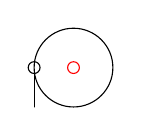
\begin{tikzpicture}[baseline=(current bounding box.center),yscale=-1,scale=0.5,every path/.style={join=round,cap=round},xscale=1]
    \draw (0.000000,0.000000) -- (0.000000,0.500000);
    \draw (0.000000,0.500000) -- (0.000000,1.000000);
    \filldraw[fill=white] (0,0) circle(0.15);
    \draw (1,0) circle (1);
    % \node[circle,draw=red,fill=white,inner xsep=1cm,inner ysep=0] at (1,0) {};
    \node[circle,draw=red,inner xsep=0.075cm,inner ysep=0cm] at (1,0) {};
  \end{tikzpicture}
\]

% \[
  % \twocell{(1->2)[none]}
% \]

% empty:
% \[
  % \twocell{}
% \]

% \[
  % \twocell{(0->2)[sqcap]}
% \]

% \[
  % \twocell{(cap * 1) * (1 * (0->0)[circle,fill=lightgray] * 2) * (cup * 1)}
% \]

% \[
  % \twocell[xscale=2.]{(mu * 1) * (2->1)[rectangle,height=2]}
% \]

% \[
  % \twocell{(mu * space2["\hat x"] * mu)}
% \]

% \[
  % \twocell{dots * mu}
% \]

% \[
  % \fbox{\twocell{dots * mu}}
% \]

% \[
  % \twocell{(1 * space2[height=0] * 2) * (dots * 1) * ((2->1)[triangle,"\mu",labelheight=1.5,position=0.1] * 1[height=2]) * mu}
% \]

% \[
  % \twocell{(1->1)[fill=red,righthalfcircle]}
% \]

% \[
  % \twocell{((2->2)[braidr'] * 2) * 4}
% \]

% \[
  % \twocell{dots * (2->6)[rectangle,"\psi"] * (dots * mu * dots)}
% \]

% \[
  % \twocell{(eta * eta * eta) * (1 * dots)}
% \]

% \[
  % \twocell{
    % (delta * 2) *
    % (dots * 2) * (mu * 2)}
  % \twocell{
    % (2 * cup * 2)
    % * (dots * dots)
    % *
    % (2 * cap * 2)
  % }
% \]

% \[
  % \twocell{vdots}
  % ==
  % \]

% \[
  % \twocell{((0->1) * (0->1)["a"]) * mu * (1->1)[rectangle,"f"]}
% \]

% \twocell{(1 * dots) * (sigma * psi) * (1 * dots)}

% we are here:
% \[
  % \twocell{(eta * (1->1)["f"]) * (1 * eps)}
% \]

% \[
  % \twocell{(eta * eta) * (1 * eps * 1) * ((2->0)[cup])}
% \]

% \[
  % \twocell{label[down,"x","y"] * 2 * mu * delta}
% \]

% \[
  % \twocell{(1 * delta) * (mu * 1) * (1 * delta[name=DELTA,"d"])}
% \]


% \[
  % \twocell{(2 * J- * (1 -> 1)[name=X,"x"])}
% \]

% \[
  % \twocell[scale=.5,thick]{(3 -> 2)}
  % \]

% \[
  % \twocell{((2 -> 1)[mergeleft] * (2 -> 1)[mergeright]) * ((1 -> 2)[mergeleft] * (1 -> 2)[mergeright])}
  % \]

% \[
  % \twocell{((2 -> 1)[cup])}
  % \]

% \[
  % \twocell{1*1*1*1}
  % =
  % \twocell{(1 -> 0)*0*0*0}
% \]

% \[
  % \twocell{(mu * 1) * mu}
% \]
% and
% \[
  % \twocell{(eta *0 eta)
    % *
    % mu}
% \]

% TESTING

% \expandafter\newcommand\csname cul8r\endcsname{Goodbye!}
% I said, ``\csname cul8r\endcsname''.

% \defsatexfig5{hello}
% J'ai dit \usesatexfig5 et \usesatexfig0
\end{document}
